\documentclass{article}
\usepackage{graphicx}
\graphicspath{ {./img/} }
\usepackage{amsmath}
\usepackage{amsfonts}
\usepackage{amssymb}
\usepackage{mathtools}
\usepackage[dvipsnames]{xcolor}
\usepackage{tkz-euclide}
\usepackage{tikz}
\usepackage{subfiles}
\usepackage{pgfplots}
\usepackage{setspace}
\pgfplotsset{compat=1.15}
\usepackage{mathrsfs}
\usetikzlibrary{arrows}
\usepackage[left=1.5cm, right=1.5cm, top=1.5cm, bottom=1.5cm]{geometry}
\pgfplotsset{compat = newest}
\usepackage[normalem]{ulem}

\onehalfspacing % 1.5

\definecolor{ududff}{rgb}{0.30196078431372547,0.30196078431372547,1.}
\definecolor{ccqqqq}{rgb}{0.8,0.,0.}
\definecolor{qqwuqq}{rgb}{0.,0.39215686274509803,0.}
\definecolor{xdxdff}{rgb}{0.49019607843137253,0.49019607843137253,1.}


\graphicspath{ {./img/} }

\usepackage{hyperref}
\hypersetup{
    colorlinks,
    citecolor=black,
    filecolor=black,
    linkcolor=black,
    urlcolor=black
}

\title{Sistemi di Elaborazione}
\author{Andrea Bellu}
\date{2023/2024}

\begin{document}

\maketitle

\tableofcontents
\newpage

\section{Introduzione}
La macchina di Turing è una macchina teoretica che può essere usata per simulare il funzionamento di un computer. Turing $\iff$ Funzione Ricorsiva (teoria logica dell'aritmetica).\\
Logica: Logica del Primo Ordina $\implies$ Logica Proposizionale\\
Teoria: Teoria Logica.\\
Ci sono cose che un sistema di elaborazione non può fare.\\
Tutto ciò finisce all'interno delle CPU (Central Processing Unit).\\
Parleremo di Cache e dei cenni su due architetture, quali: GPU e Quantum Computing.\\
Una volta costruito l'hardware, bisogna scrivere il software, degli algoritmi per gestirlo.

\section{Connettivi Proposizionali}
La logica proposizionale è un metodo per calcolare il valore di verità di una proposizione. Il simbolo di vero è $1$, mentre il simbolo di falso è $0$.

\subsection{Negazione NOT}
Se A è una frase $\neg A$ è la negazione di A. Quando A è vera, $\neg A$ è falsa e viceversa.
\begin{center}
    \begin{tabular}{|c|c|}
        \hline
        A & $\neg A$ \\
        \hline
        1 & 0 \\
        0 & 1 \\
        \hline
    \end{tabular}
\end{center}
\subsection{Congiunzione AND}
Se A e B sono frasi, $A \land B$ è la congiunzione di A e B. $A \land B$ è vera solo se entrambe A e B sono vere.
\begin{center}
    \begin{tabular}{|c|c|c|}
        \hline
        A & B & $A \land B$ \\
        \hline
        1 & 1 & 1 \\
        1 & 0 & 0 \\
        0 & 1 & 0 \\
        0 & 0 & 0 \\
        \hline
    \end{tabular}
\end{center}
\subsection{Disgiunzione OR}
La disgiunzione delle frasi A e B è indicata dal simbolo $A \lor B$. $A \lor B$ è vera se almeno una delle due frasi è vera.
\begin{center}
    \begin{tabular}{|c|c|c|}
        \hline
        A & B & $A \lor B$ \\
        \hline
        1 & 1 & 1 \\
        1 & 0 & 1 \\
        0 & 1 & 1 \\
        0 & 0 & 0 \\
        \hline
    \end{tabular}
\end{center}
\subsection{Implicazione condizionale o materiale}
Date due frasi, A e B, l'implicazione condizionale è indicata con $A \implies B$. L'implicazione è falsa solo quando A è vera e B è falsa. Si può leggere come "se A allora B". Per capire l'idea che sta alla base del condizionale, si pensi alla frase:
\begin{center}
    "Per ogni $x$, se $x$ è un numero intero positivo dispari, allora $x^2$ è un numero intero positivo dispari."
\end{center}

\begin{center}
    \begin{tabular}{|c|c|c|}
        \hline
        A & B & $A \implies B$ \\
        \hline
        1 & 1 & 1 \\
        1 & 0 & 0 \\
        0 & 1 & 1 \\
        0 & 0 & 1 \\
        \hline
    \end{tabular}
\end{center}
\subsection{Bicondizionale}
Il bicondizionale è indicato con $A \iff B$. Il bicondizionale è vero se entrambe le frasi sono vere o entrambe le frasi sono false.
\begin{center}
    \begin{tabular}{|c|c|c|}
        \hline
        A & B & $A \iff B$ \\
        \hline
        1 & 1 & 1 \\
        1 & 0 & 0 \\
        0 & 1 & 0 \\
        0 & 0 & 1 \\
        \hline
    \end{tabular}
\end{center}
\subsection{Forme enunciative FINIRE}



\subsection{Convenzioni tra parentesi}
\begin{figure}
    \centering
    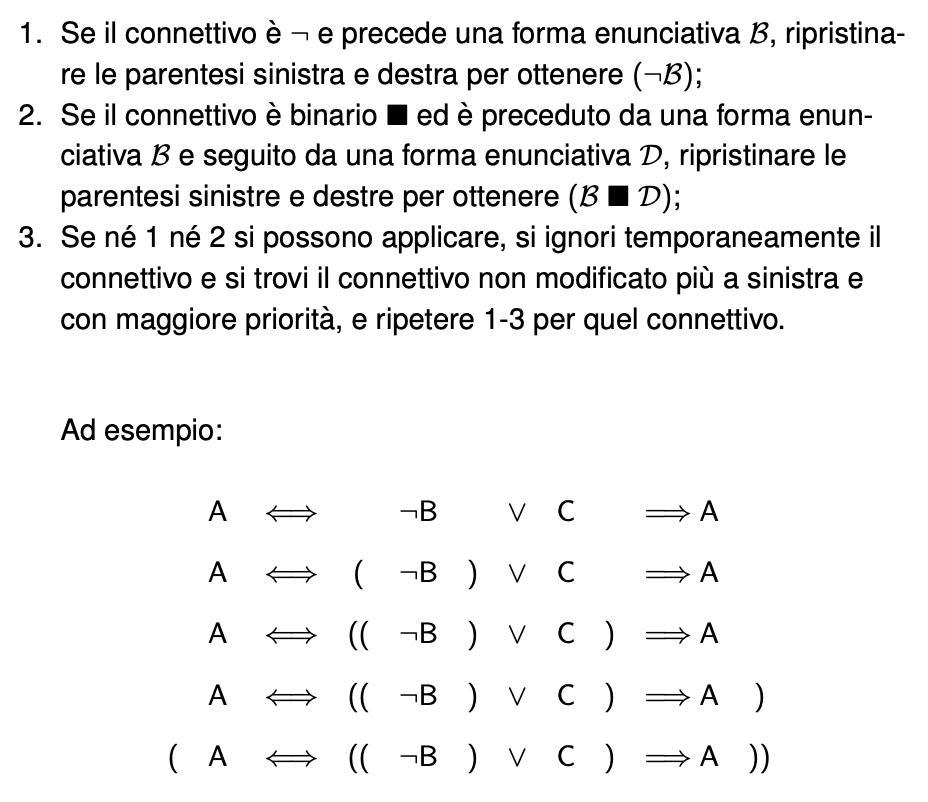
\includegraphics[width=0.7\textwidth]{Screenshot 2024-02-21 at 11.37.14.png}
    \caption{Convenzioni tra parentesi}
    \label{fig:parenthesis}
\end{figure}

\subsection{Esercizio 1}
\begin{figure}
    \centering
    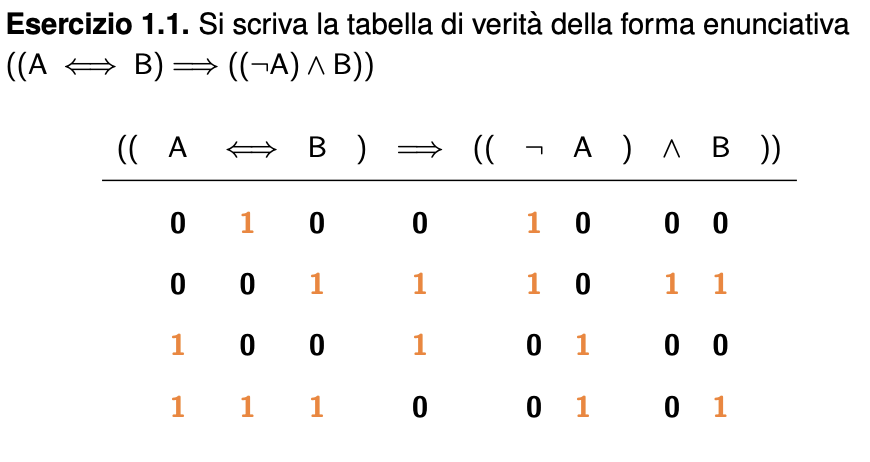
\includegraphics[width=0.7\textwidth]{Screenshot 2024-02-21 at 11.41.48.png}
    \caption{Esercizio 1}
    \label{fig:ex1}
\end{figure}
\subsection{Forma enunciativa soddisfacibile}
Diremo che una forma enunciativa è soddisfacibile se è vera per qualche assegnazione di valori di verità 1.

\section{Tautologie e Contraddizioni}
\subsection{Tautologia}
Una forma enunciativa è una tautologia se è vera per ogni assegnazione di valori di verità.\\
\begin{center}
    \begin{tabular}{|c|c|c|}
        \hline
        A & B & $A \lor \neg A$ \\
        \hline
        1 & 0 & 1 \\
        0 & 1 & 1 \\
        \hline
    \end{tabular}
\end{center}

\subsection*{Esercizio 2.2}
\begin{figure}[h!]
    \centering
    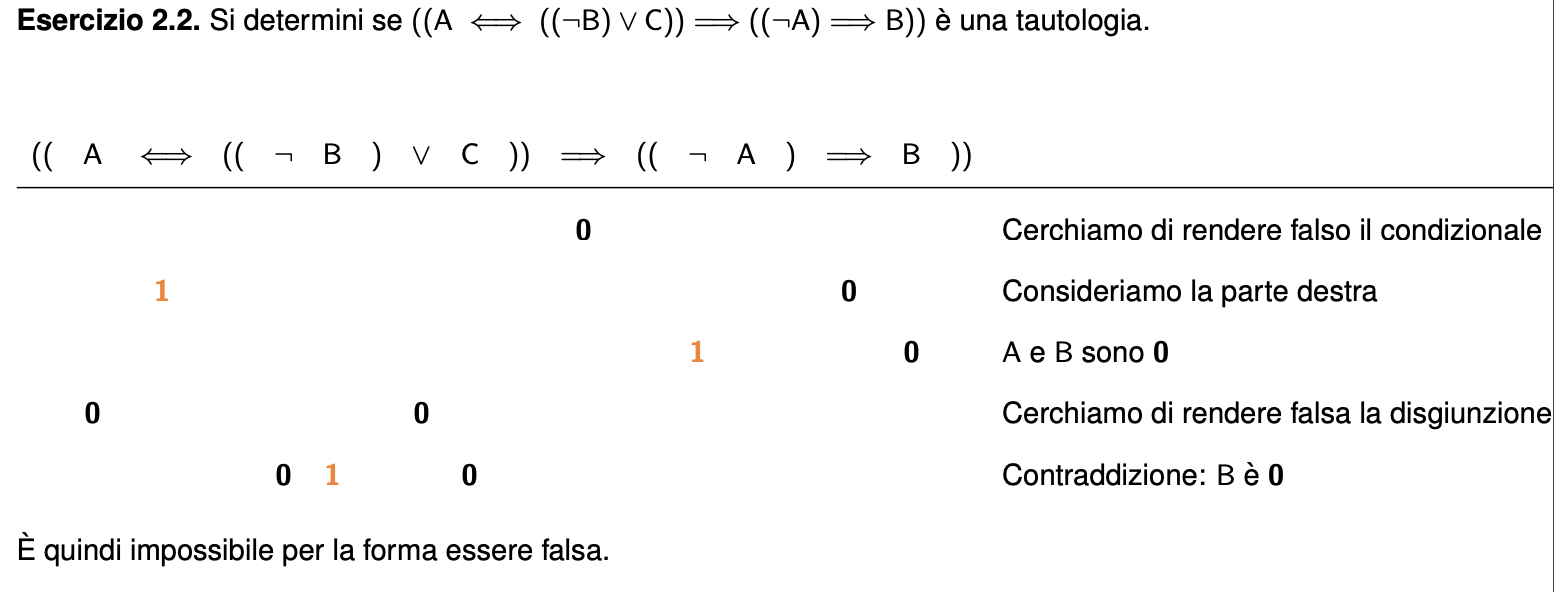
\includegraphics[width=0.7\textwidth]{Screenshot 2024-02-21 at 11.46.14.png}
    \caption{Esercizio 2.2}
    \label{fig:ex2.2}
\end{figure}

\subsection{Contraddizione}
Una forma enunciativa è una contraddizione se è falsa per ogni assegnazione di valori di verità.\\
\begin{center}
    \begin{tabular}{|c|c|c|}
        \hline
        A & B & $A \land \neg A$ \\
        \hline
        1 & 0 & 0 \\
        0 & 1 & 0 \\
        \hline
    \end{tabular}
\end{center}

\section{Implicazione ed Equivalenza logica}
\subsection{Implicazione logica}
B implica logicamente C o analogamente C è una conseguenza logica di B $\iff$ ogni assegnamento di verità alle lettere enunciative di B e C che rende B vera (con valore 1), rende vera anche C.

\subsection{Equivalenza logica}
B e C sono logicamente equivalenti se e solo se B e C hanno lo stesso valore di verita per ogni assegnazione di valori di verita di ogni lettera enunciativa di B e C.

\section{Connettivi e porte logiche}
Ogni funzione di verita` e generata da una forma enunciativa che coinvolge i `
connettivi $\neg, \land, \lor$.

Ogni funzione di verità può essere generata da una forma enunciativa che coinvolge i connettivi $\neg, \land, \lor$.

\subsection*{NOR joint denial}
\begin{center}
    \begin{tabular}{|c|c|c|}
        \hline
        A & B & $A \downarrow B$ \\
        \hline
        1 & 1 & 0 \\
        1 & 0 & 0 \\
        0 & 1 & 0 \\
        0 & 0 & 1 \\
        \hline
    \end{tabular}
\end{center}

\subsection*{NAND}
\begin{center}
    \begin{tabular}{|c|c|c|}
        \hline
        A & B & $A | B$ \\
        \hline
        1 & 1 & 0 \\
        1 & 0 & 1 \\
        0 & 1 & 1 \\
        0 & 0 & 1 \\
        \hline
    \end{tabular}
\end{center}

Le porte logiche sono HW fondamentale su cui sono costruiti i computer.
\begin{figure}[h!]
    \centering
    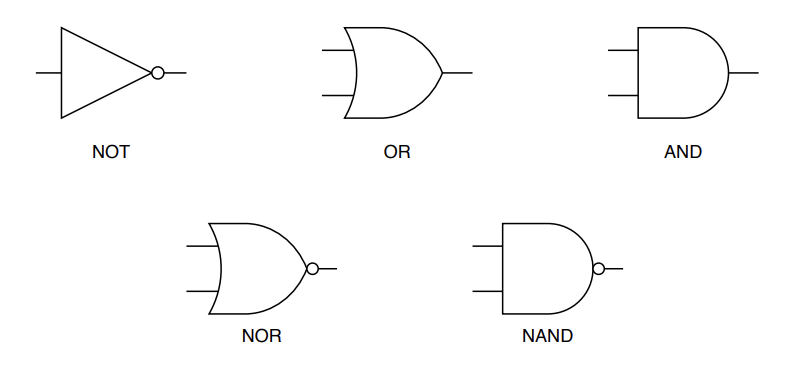
\includegraphics[width=0.7\textwidth]{porte_logiche.png}
    \caption{Porte logiche}
\end{figure}

\subsection{Transistor}
\begin{figure}[h!]
    \centering
    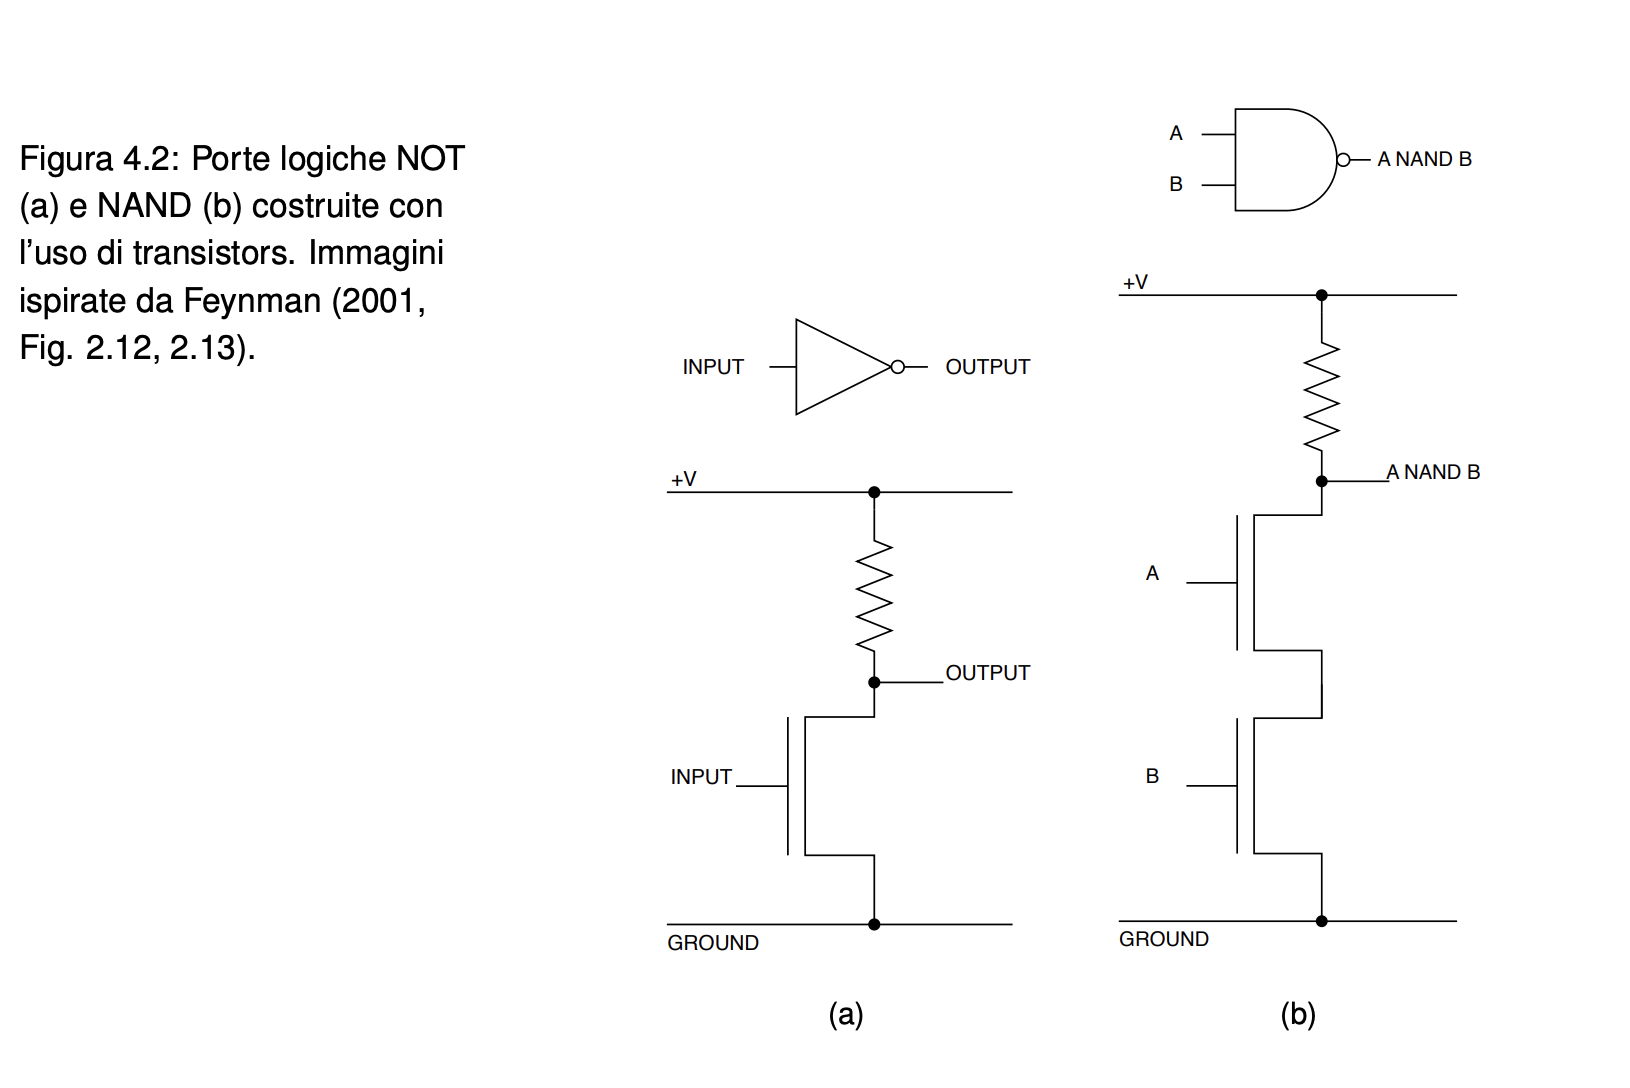
\includegraphics[width=0.7\textwidth]{trans.png}
    \caption{Transistor}
\end{figure}

\section{Forme normali e implicazionie ogica via risoluzione}


\end{document}
